\section{Participatory Design}
In the following, the users can also be described with the terms \textit{students} and \textit{artists}.

%NOTE: terms we use: scene camera vs framing camera
%Framing: influence point + camera + connection
%Player path

An initial mockup of the tool's interface and functionality was created internally. The mockup had the interface all gathered in one window to keep the design minimalist. However, in search of a better design, we included the end-users in the process going forward (see Figure \ref{fig:mockup}).

To ground our design work, we were interested in learning more about our users and how they envisioned the finished product. Therefore, three participatory exercises were conducted \footnote{The exercises were video documented, except for one artist and half of the footage from another artist in the first exercise}. The first of which was done to know their general workflow when working with cameras in the tools they, namely Maya and Unity. Secondly, we wanted to know which features they requested and how they envisioned the finished tool. Finally, they tried using a prototype of the camera tool based on their initial design and feature requests.


\begin{figure}[htbp]
\centering
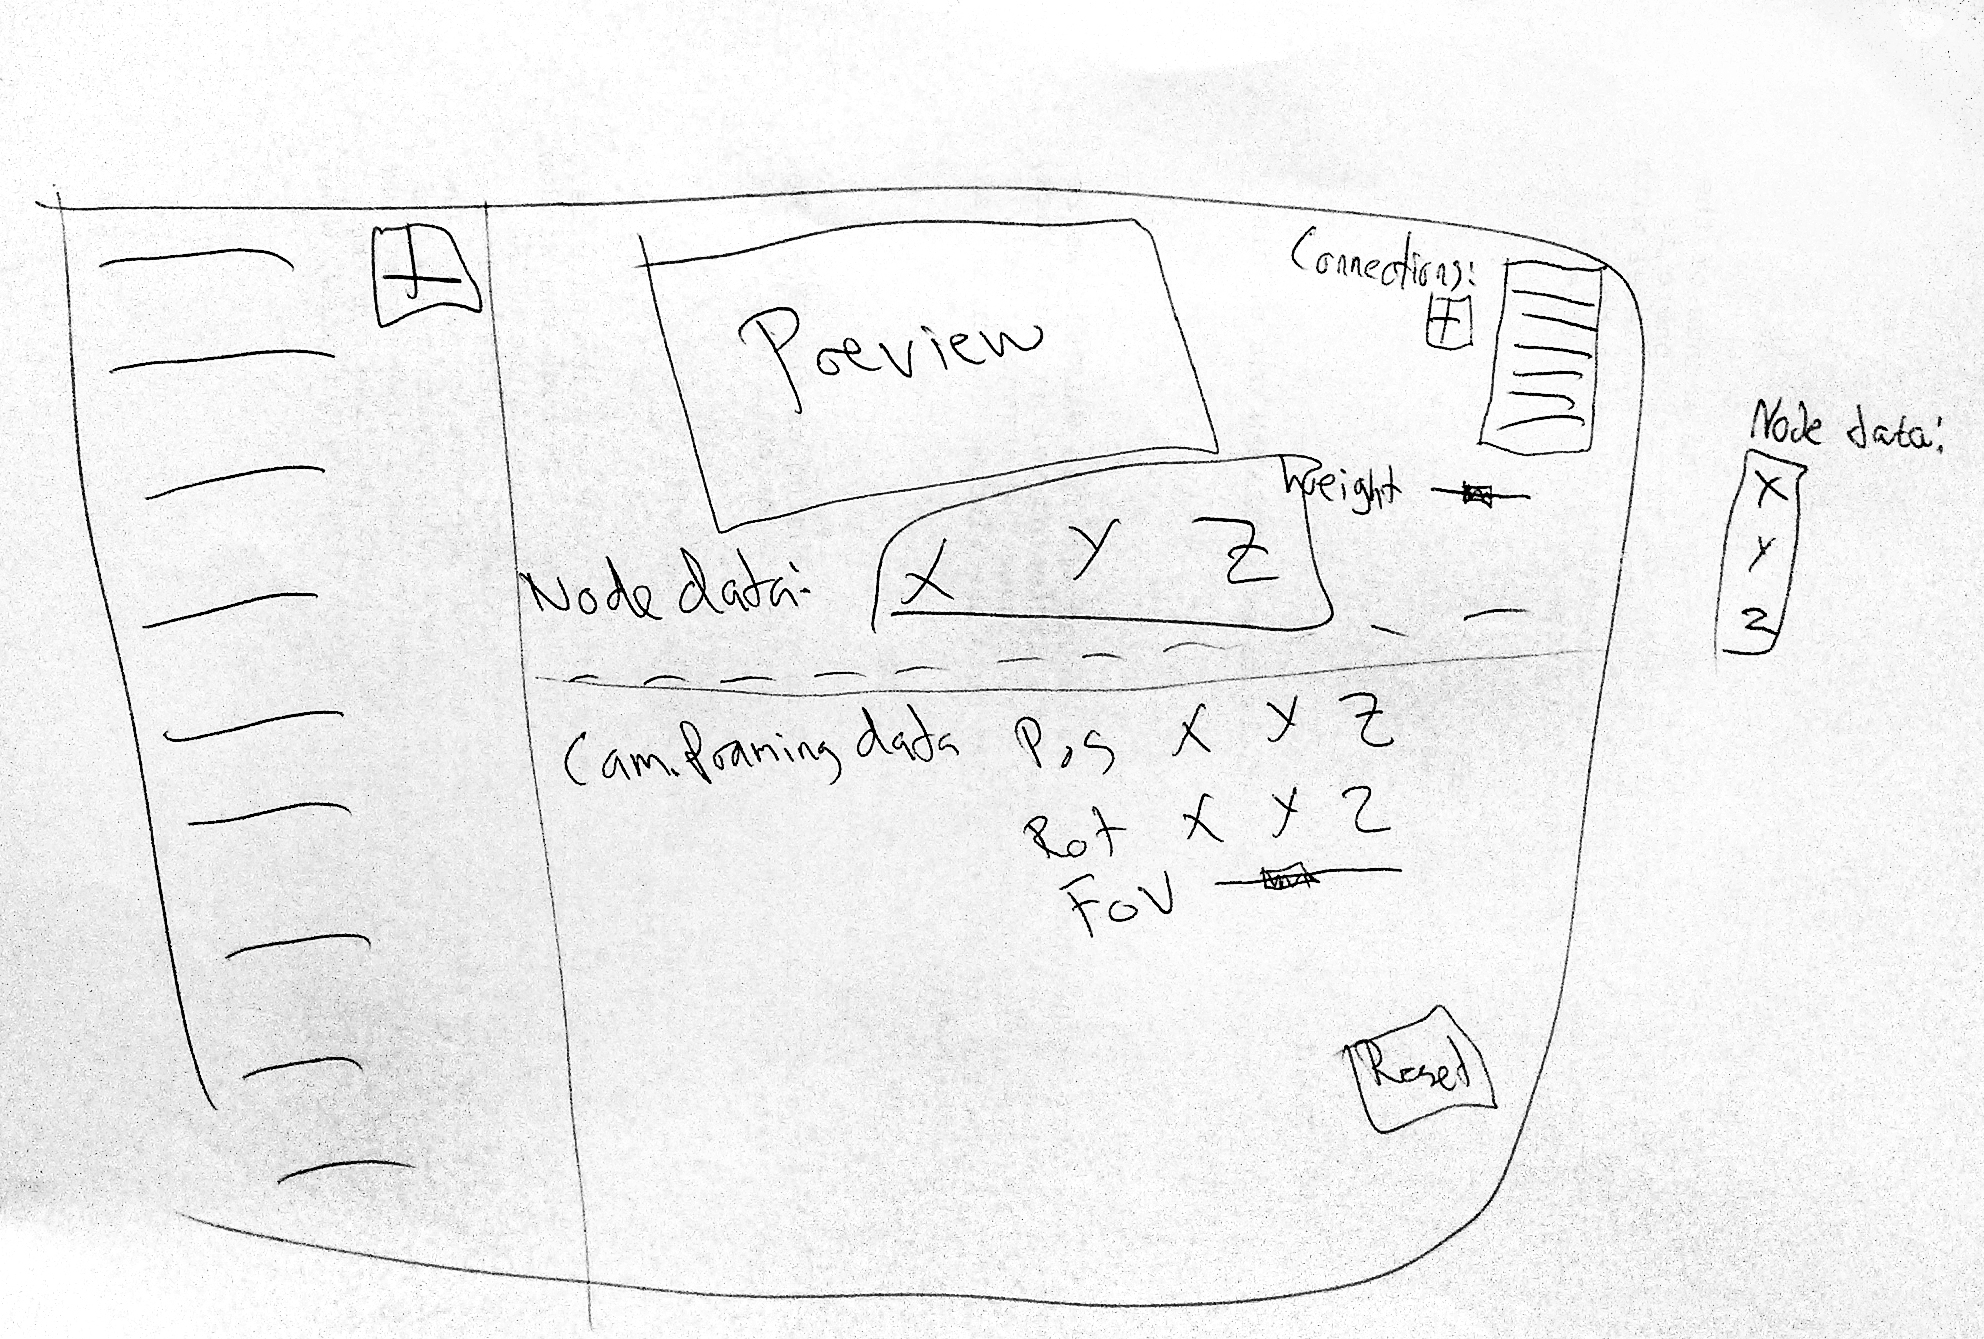
\includegraphics[width=0.50\textwidth]{Pics/InitialMockup}
\caption{The initial concept was to have all the feature tools inside one big window. Early on it was observed that all of the students from The Animation Workshop use a dual-monitor setup, they could then dedicate one monitor to the camera tool.}
\label{fig:mockup}
\end{figure}

\subsection{Exercise 1: Knowledge of tools} \label{exerciseOne}
An artist and a facilitator sat down in front of the artist's work area. The facilitator then asked the artist to show him how he would animate a camera around an object in Maya (see Figure \ref{fig:mads_dual}). This included keyframing and how to change the camera settings for each keyframe. This was done to get an idea of how they usually work. If our camera tool should be successful at helping these artists, it should mimic some of the same behaviour that Maya has. It seemed ideal that the users should be able to utilize their previously-gained knowledge from Maya wherever applicable.

\begin{figure}[htbp]
\centering
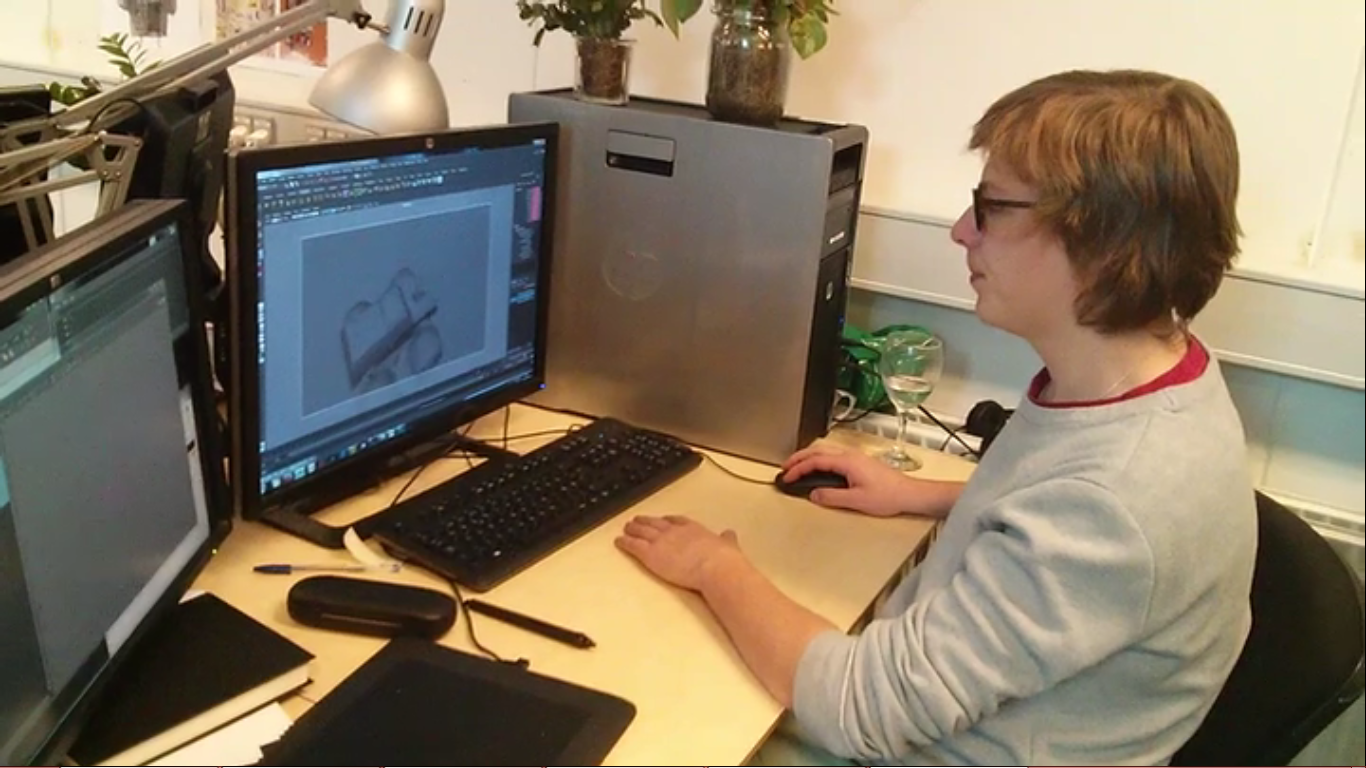
\includegraphics[width=0.3\textwidth]{Pics/Mads_dual}
\caption{All the students at The Animation Workshop work with a dual monitor setup.}
\label{fig:mads_dual}
\end{figure}

After this, the facilitator and artist switched to Unity where he was tasked with moving around in the scene and then to create basic objects such as cubes and spheres, as well as positioning the camera. The purpose of this was to get an understanding of how skilled they are at using Unity - moving around the scene, rotating and translating objects etc. This was done with another two artists as well. The first section of the exercise, the Maya part, was the same for all three artists, but the questions and tasks changed in the last section as the facilitator gained new knowledge about their skill level.

It was discovered that none of the artists knew how to use a standard Unity feature that lets the player fly around with the scene camera as if they were playing a first-person game ("Flythrough Mode", \cite{unity_flyMode}). The artist were excited about the discovery of this feature. One artist perceived the standard way of moving around in Unity as confusing, while another stated that the way of moving the camera is exactly like in Maya. After testing this ourselves, we concluded that the movement controls in Maya and Unity are indeed very similar (except for the "Flythrough Mode"), which means that the artists should ideally be comfortable with navigating in either of the applications.

\subsection{Exercise 2: Paper prototyping}
The artists were given a blank sheet of paper and a pen and was tasked to draw and write about the camera tool, as they envisioned it in a free-form approach. They then explained what they did and they had a discussion about it. There were no strict requirements of how they approached the task, so some focused a lot on feature requires, while others were more interested in fundamental workflow and user interfaces. This was done with four artists in total.

After this, the same four artists were placed at a desk, one by one, where a variety of labels were laid out in front of them (see Figure \ref{fig:labels}). These labels were marked as different sliders, buttons, windows, field parameters, camera settings, etc. The labels were primarily based on the basic building blocks of Unity's user interface, as well as some of the observations from the first exercise where the users talked about how they worked with Maya.

\begin{figure}[htbp]
\centering
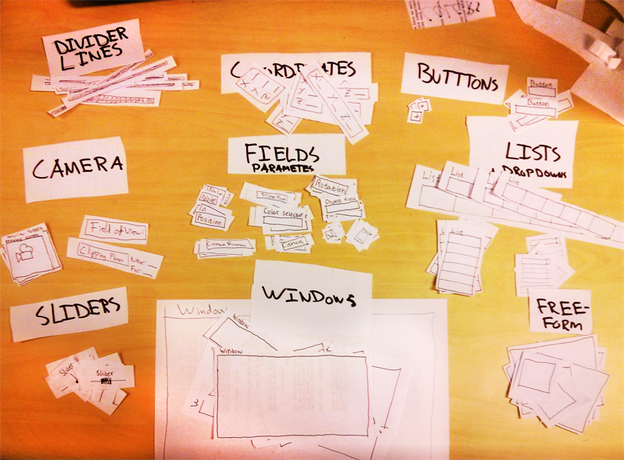
\includegraphics[width=0.3\textwidth]{Pics/labels}
\caption{The users were asked to design their "dream program" by using paper labels as building blocks. They were also allowed to draw their own components if necessary.}
\label{fig:labels}
\end{figure}

All artists wanted basic features like translation, rotation, field of view of the camera, as well as a curve editor to change the interpolation between two cameras. After these features, all the artists diverted in their designs. All the designs were discussed internally and main points and ideas were extracted from them. These findings were used as the foundation of the tool's design. However, the foundation for the program was not strictly based on the artists ideas and requirements; instead, we tried to extract some more general requests of what they as artists actually need. It was important to keep in mind that working in an interactive medium such as game development was a new experience for the users.

A slider that could be used to interpolate between two camera framings in a preview window is an example of an idea that was discarded by us. The artist wanted two preview windows of the camera framing, as well as a preview window of the interpolation, which the slider would manipulate. His idea was similar to a DJ turntable. After discussing it internally, we concluded that this idea would make the interface too elaborate, but the idea of being able to preview your changes quickly was kept.

% put into appendixs
%See Figures \ref{fig:morten_requirements} and \ref{fig:mads_turntable}.

% morten PUT INTO APPENDIX
%\begin{figure}[htbp]
%\centering
%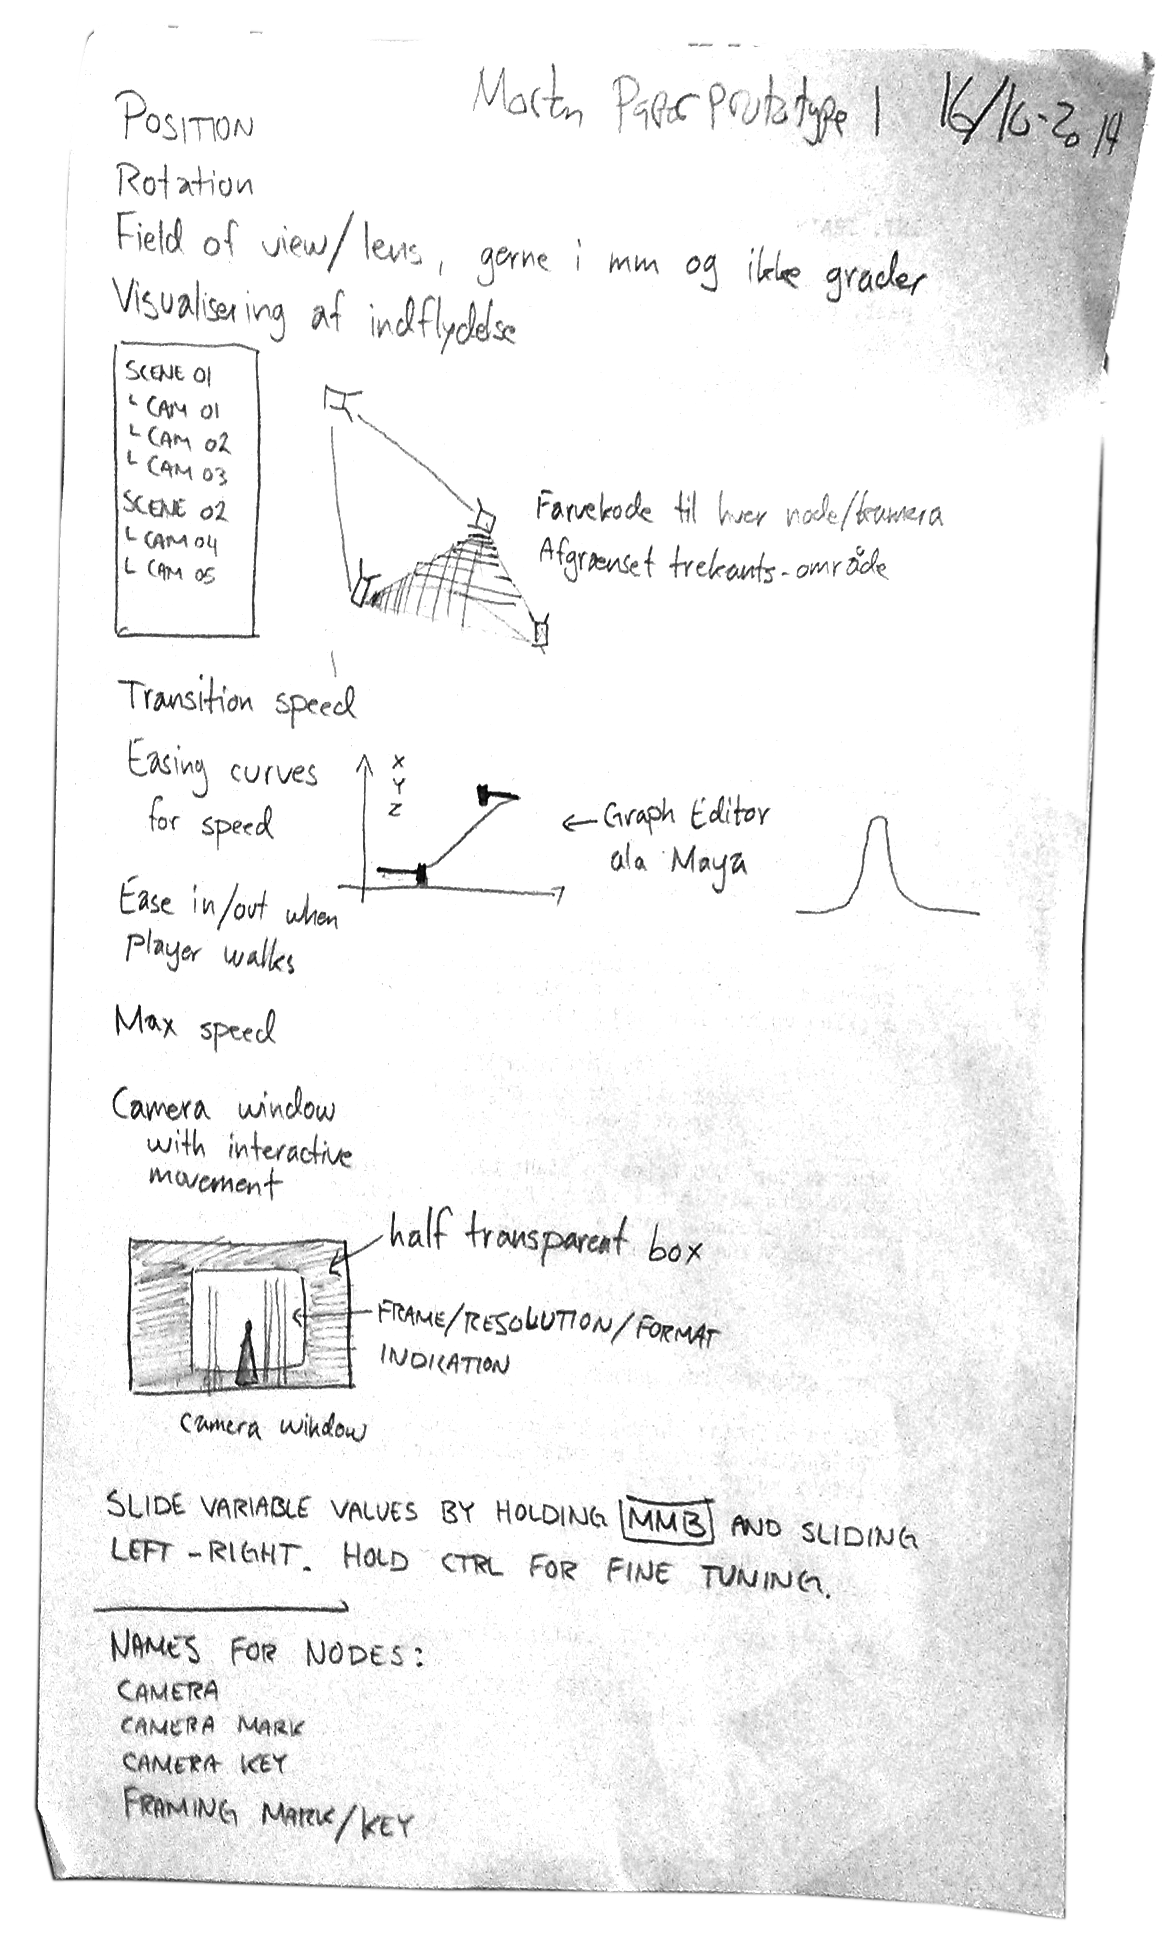
\includegraphics[width=0.50\textwidth]{Pics/Morten01}
%\caption{Feature requirements.}
%\label{fig:morten_requirements}
%\end{figure}

% mads PUT INTO APPENDIX
%\begin{figure}[htbp]
%\centering
%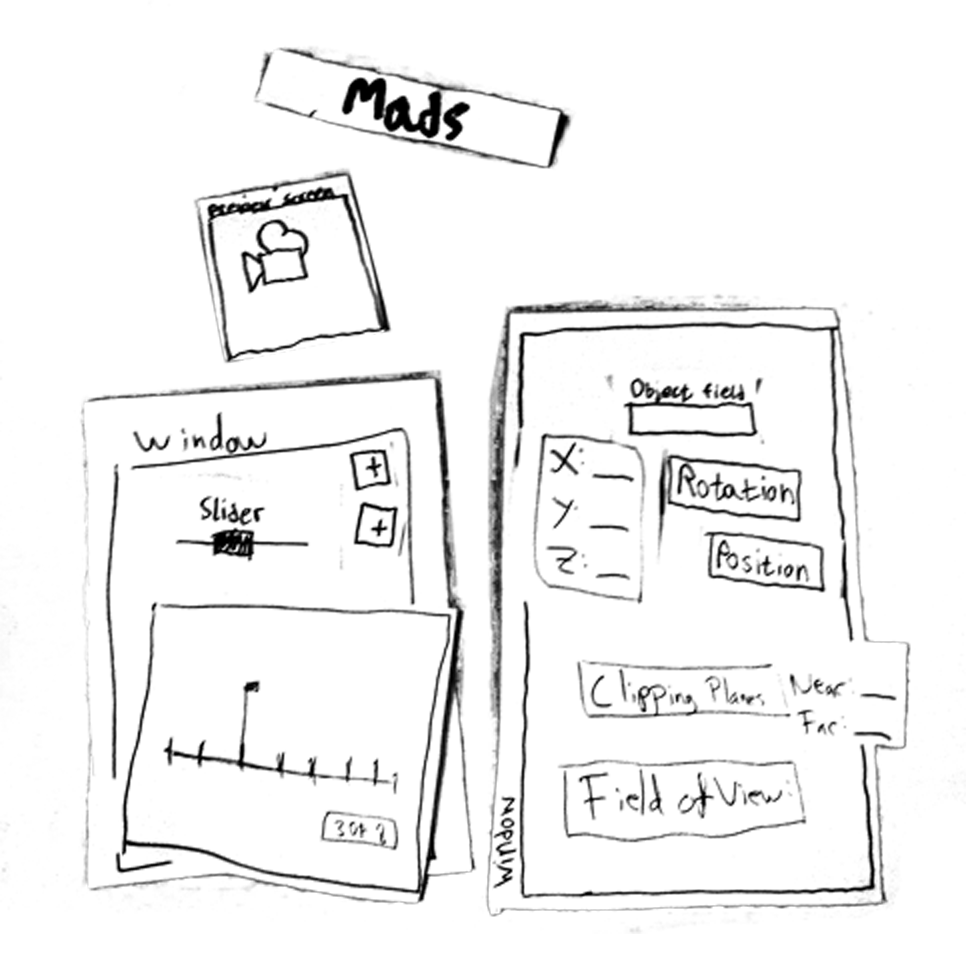
\includegraphics[width=0.50\textwidth]{Pics/Mads01}
%\caption{Turntable concept.}
%\label{fig:mads_turntable}
%\end{figure}

\subsection{Summary of Findings}
It was found that the students are comfortable working in Maya and use it as their main reference point when working in 3D applications. The overall design of the camera tool should take this into considerations to make the transition from Maya to Unity as smooth as possible.

Some of the more concrete findings include:
\begin{itemize}
\item Basic camera manipulation: translation, rotation, field of view, lenses, easing, etc.
\item Camera modes
\begin{itemize}
\item Look through the camera when positioning it
\item Aim point
\item Domains areas
\item Toggle camera to either follow or be static
\end{itemize}
\item Curves and graph editors
\item Hotkeys (e.g., set new camera with "S")
\item Easy to get an overview and navigate between framings
\item Tool should be optimal for dual-monitor setups and easy to customize window layout (draggability)
\item Optimal workflow
\begin{itemize}
\item Real-time preview: Be able to move a puppet-like character around to get a feel of the interpolation (similar to the yellow Google "pegman" in Street View)
\item Having an easy-to-access list of all framings
\item 2D overview of the map with all camera keys/markers
\item When looking through the camera, have transparent border (like in Maya)
\item In camera preview, show what camera is currently 'dominant' (how much weight each camera is pulling)
\end{itemize}
\end{itemize}

\subsection{Exercise 3: First iteration}
After having completed the two exercises, we started developing a rough prototype in Unity (see Figure \ref{fig:prototype}). This iteration included basic functionality to make it possible to test and get feedback as quickly as possible. During one of their daily SCRUM meetings, we presented the tool, as well as providing them a short manual (SEE APPENDIX A).


\begin{figure}[htbp]
\centering
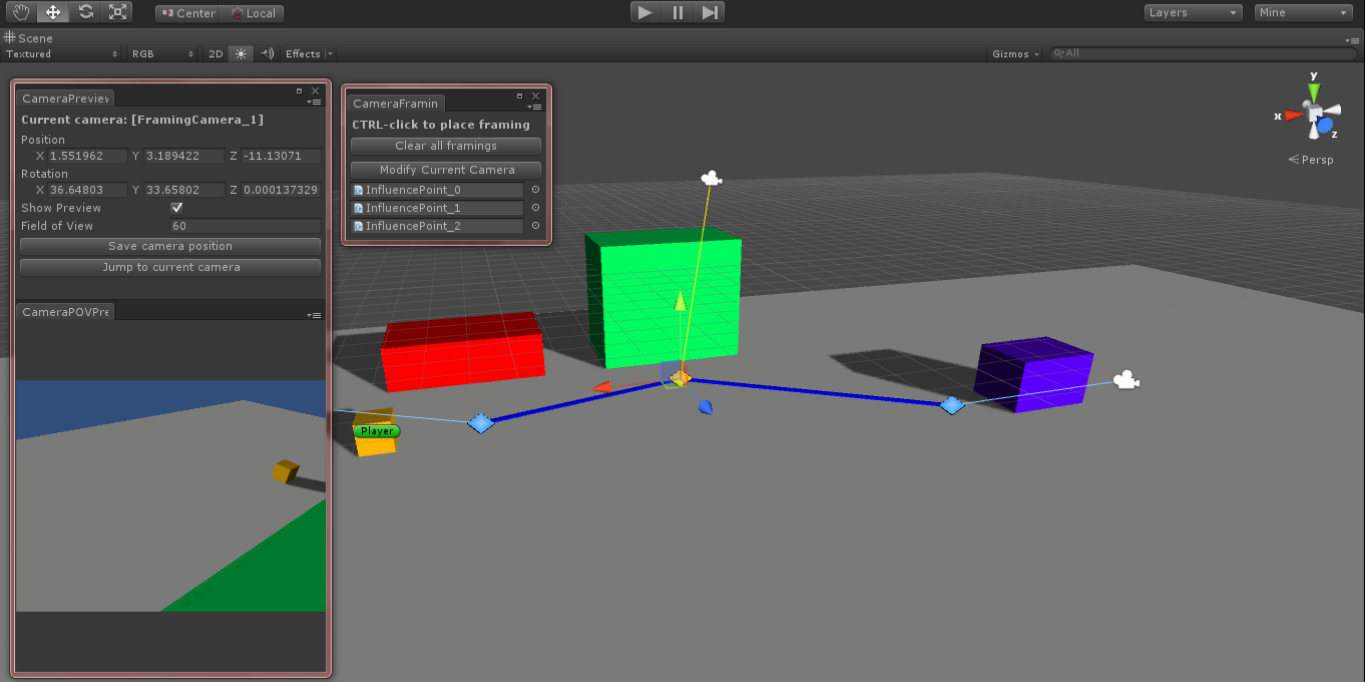
\includegraphics[width=0.50\textwidth]{Pics/MainSetup}
\caption{Rough prototype with basic camera manipulation.}
\label{fig:prototype}
\end{figure}

Three artists tried it out for 10-40 minutes each. They got a chance to try out the tool, as well as expressing their overall opinion about how they preferred the workflow to be.

The facilitator gave the artist small tasks like "Can you place Framings along this paths?" and "Can you try and set the Framing's camera settings as you'd like?". This exercise was semi-structured, and not all questions were predetermined; some was thought up as the exercise went on.

Over the course of the exercise, some key points was discovered through observation or discussion with the artist. The biggest piece of feedback revolved how the users are supposed to place the virtual camera in the scene. Initially, users were supposed to use Unity's "Flythrough Mode" (see Section \ref{exerciseOne}) and place the camera as they liked. Then, they should press the "Save camera position" button (see Figure \ref{fig:prototype}). However, some users were confused about this, since they thought that they now they continuously looked through the camera's point of view, i.e. if they moved around after they'd pressed the button, the framing camera should be changed as well. This was not how the system worked, since it simply just saved the scene camera's position to the framing camera whenever the button was pressed. In other words, the users mental models didn't fit with how the tool worked.
